\documentclass[border=4pt]{standalone}
\usepackage{amsmath}
\usepackage{tikz}
\usepackage{pgfplots}
\pgfplotsset{compat=1.18}
\usetikzlibrary{arrows.meta}
\begin{document}
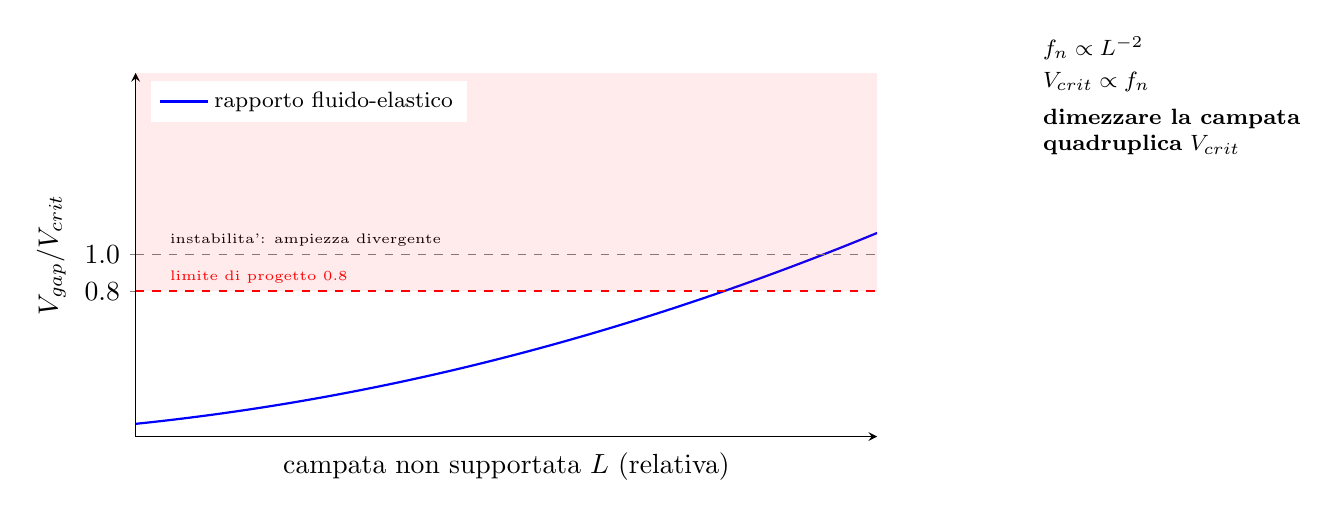
\begin{tikzpicture}
\begin{axis}[
  width=11cm, height=6.2cm,
  xlabel={campata non supportata $L$ (relativa)},
  ylabel={$V_{gap}/V_{crit}$},
  xtick=\empty, ytick={0.8,1.0}, yticklabels={0.8,1.0},
  axis lines=left,
  ymin=0, ymax=2.0, xmin=0.5, xmax=2.0,
  legend style={font=\footnotesize, at={(0.02,0.98)}, anchor=north west, draw=none},
]
\addplot[thick,blue,domain=0.5:2.0,samples=60]{0.28*x^2};
\addlegendentry{rapporto fluido-elastico}
\draw[dashed,red,thick] (axis cs:0.5,0.8) -- (axis cs:2.0,0.8);
\node[font=\tiny,red,anchor=west] at (axis cs:0.55,0.88) {limite di progetto 0.8};
\draw[dashed,gray] (axis cs:0.5,1.0) -- (axis cs:2.0,1.0);
\node[font=\tiny,anchor=west] at (axis cs:0.55,1.08) {instabilita': ampiezza divergente};
\fill[red,opacity=0.08] (axis cs:0.5,0.8) rectangle (axis cs:2.0,2.0);
\end{axis}
\node[font=\footnotesize,align=left,anchor=north west] at (11.4,5.2)
  {$f_n \propto L^{-2}$\\[2pt]$V_{crit}\propto f_n$\\[4pt]\textbf{dimezzare la campata}\\\textbf{quadruplica} $V_{crit}$};
\end{tikzpicture}
\end{document}
